\documentclass[UTF8,12pt]{article}
\usepackage{ctex}
\usepackage{indentfirst}
\usepackage{color}
\usepackage{hyperref}
\usepackage{graphicx}
\usepackage{subfigure}
\usepackage{pdfpages}
\usepackage{listings}
\hypersetup{
    hidelinks,
	colorlinks=true,
	allcolors=black,
	pdfstartview=Fit,
	breaklinks=true
}

\definecolor{dkgreen}{rgb}{0,0.6,0}
\definecolor{gray}{rgb}{0.5,0.5,0.5}
\definecolor{mauve}{rgb}{0.58,0,0.82}

\lstset{ %
  language=Octave,                % the language of the code
  basicstyle=\footnotesize,           % the size of the fonts that are used for the code
  numbers=left,                   % where to put the line-numbers
  numberstyle=\tiny\color{gray},  % the style that is used for the line-numbers
  stepnumber=2,                   % the step between two line-numbers. If it's 1, each line 
                                  % will be numbered
  numbersep=5pt,                  % how far the line-numbers are from the code
  backgroundcolor=\color{white},      % choose the background color. You must add \usepackage{color}
  showspaces=false,               % show spaces adding particular underscores
  showstringspaces=false,         % underline spaces within strings
  showtabs=false,                 % show tabs within strings adding particular underscores
  frame=single,                   % adds a frame around the code
  rulecolor=\color{black},        % if not set, the frame-color may be changed on line-breaks within not-black text (e.g. commens (green here))
  tabsize=2,                      % sets default tabsize to 2 spaces
  captionpos=b,                   % sets the caption-position to bottom
  breaklines=true,                % sets automatic line breaking
  breakatwhitespace=false,        % sets if automatic breaks should only happen at whitespace
  title=\lstname,                   % show the filename of files included with \lstinputlisting;
                                  % also try caption instead of title
  keywordstyle=\color{blue},          % keyword style
  commentstyle=\color{dkgreen},       % comment style
  stringstyle=\color{mauve},         % string literal style
  escapeinside={\%*}{*)},            % if you want to add LaTeX within your code
  morekeywords={*,...}               % if you want to add more keywords to the set
}


\setlength{\parindent}{2em}

\begin{document}



\begin{center}
    \tableofcontents
\end{center}
\newpage

\section{实验目的}
\begin{enumerate}
    \item 熟悉大型数据库实验环境,以MS SQL SERVER为例
    \item 掌握DDL语句,使用DDL语句完成数据表的创建
    \item 掌握DML语句,使用DML语句完成数据的插入、修改和删除
    \item 掌握MS SQL SERVER的备份和还原
    \item 掌握MS SQL SERVER的权限分配
\end{enumerate}

\section{实验内容}
\subsection{用DDL(数据定义语句中的Create database)创建一个新数据库FlightDB,数据库文件的设置都可以使用默认值}

\subsection{用DDL(数据定义语句中的Create Table)创建三张表}
\subsubsection{航班表(hbb)}
包括如下字段:

航班号(hbh):字符型,6位定长,主码,以CZ、CA、FM开头

始发地(sfd):字符型,可变长统一编码字符型20位长,非空

目的地(mdd):字符型,可变长统一编码字符型20位长,非空

原价(YJ):整型,非空,必须>=0

\subsubsection{乘客表(Ckb)}
包括如下字段:

身份证号(sfzh):字符型,20位变长字符串,主码

姓名(xm):可变长统一编码字符型,10位长

\subsubsection{售票表(spb)}
包括如下字段:

航班号(hbh):主码 

身份证号(sfzh):主码

起飞日期(qfrq):日期时间型,非空

售票日期(sprq):日期时间型,非空,默认值为当前时间
实价(sj):整型,非空

其中:航班号为引用航班表的外码,身份证号为引用乘客表的外码。

\subsection{用DML(数据操作语句中的Insert)插入数据}
在hbb表中插入如下数据

CZ1301,北京,上海,1200

CZ1209,南京,昆明,1300

CZ1502,上海,北京,1200

CA1130,成都,北京,1800

CA1230,拉萨,广州,1500

CA1401,广州,南京,1600

\subsection{对数据库进行一次完整备份,备份名为BackupFull}

\subsection{用DML(数据操纵语句中的Insert)在乘客表和售票表中插入如下数据}

\subsection{对数据库进行一次差异备份,备份名为BackupAdd1}

\subsection{用DML(数据操纵语句中的Update)将所有目的地是北京的航班的原价提高10\%}

\subsection{用DML(数据操纵语句中的Delete)将“张飞”乘客删除,注意同时删除售票记录和乘客基本信息}

\subsection{尝试使用MS SQL Server的还原功能,还原到上一次差异备份的BackupAdd1处}

\subsection{在SQL Server中创建一个用户FlightUser,设置FlightUser用户对三张表都有查询权,但是该用户不能对乘客表和航班表进行增加、删除和修改记录,该用户对售票表能增加、删除和修改记录。然后用FlightUser登陆SQL Server,对如上权限设置进行验证}

\section{实验步骤及结果}
\subsection{DDL创建数据库}
由于文件设置使用了默认值,所以只需要使用如下语句即可创建数据库

\begin{lstlisting}[title=DDL创建数据库,frame=shadowbox]
    create database FlightDB
\end{lstlisting}

实现效果如下
\begin{figure}[htbp]
    \centering
    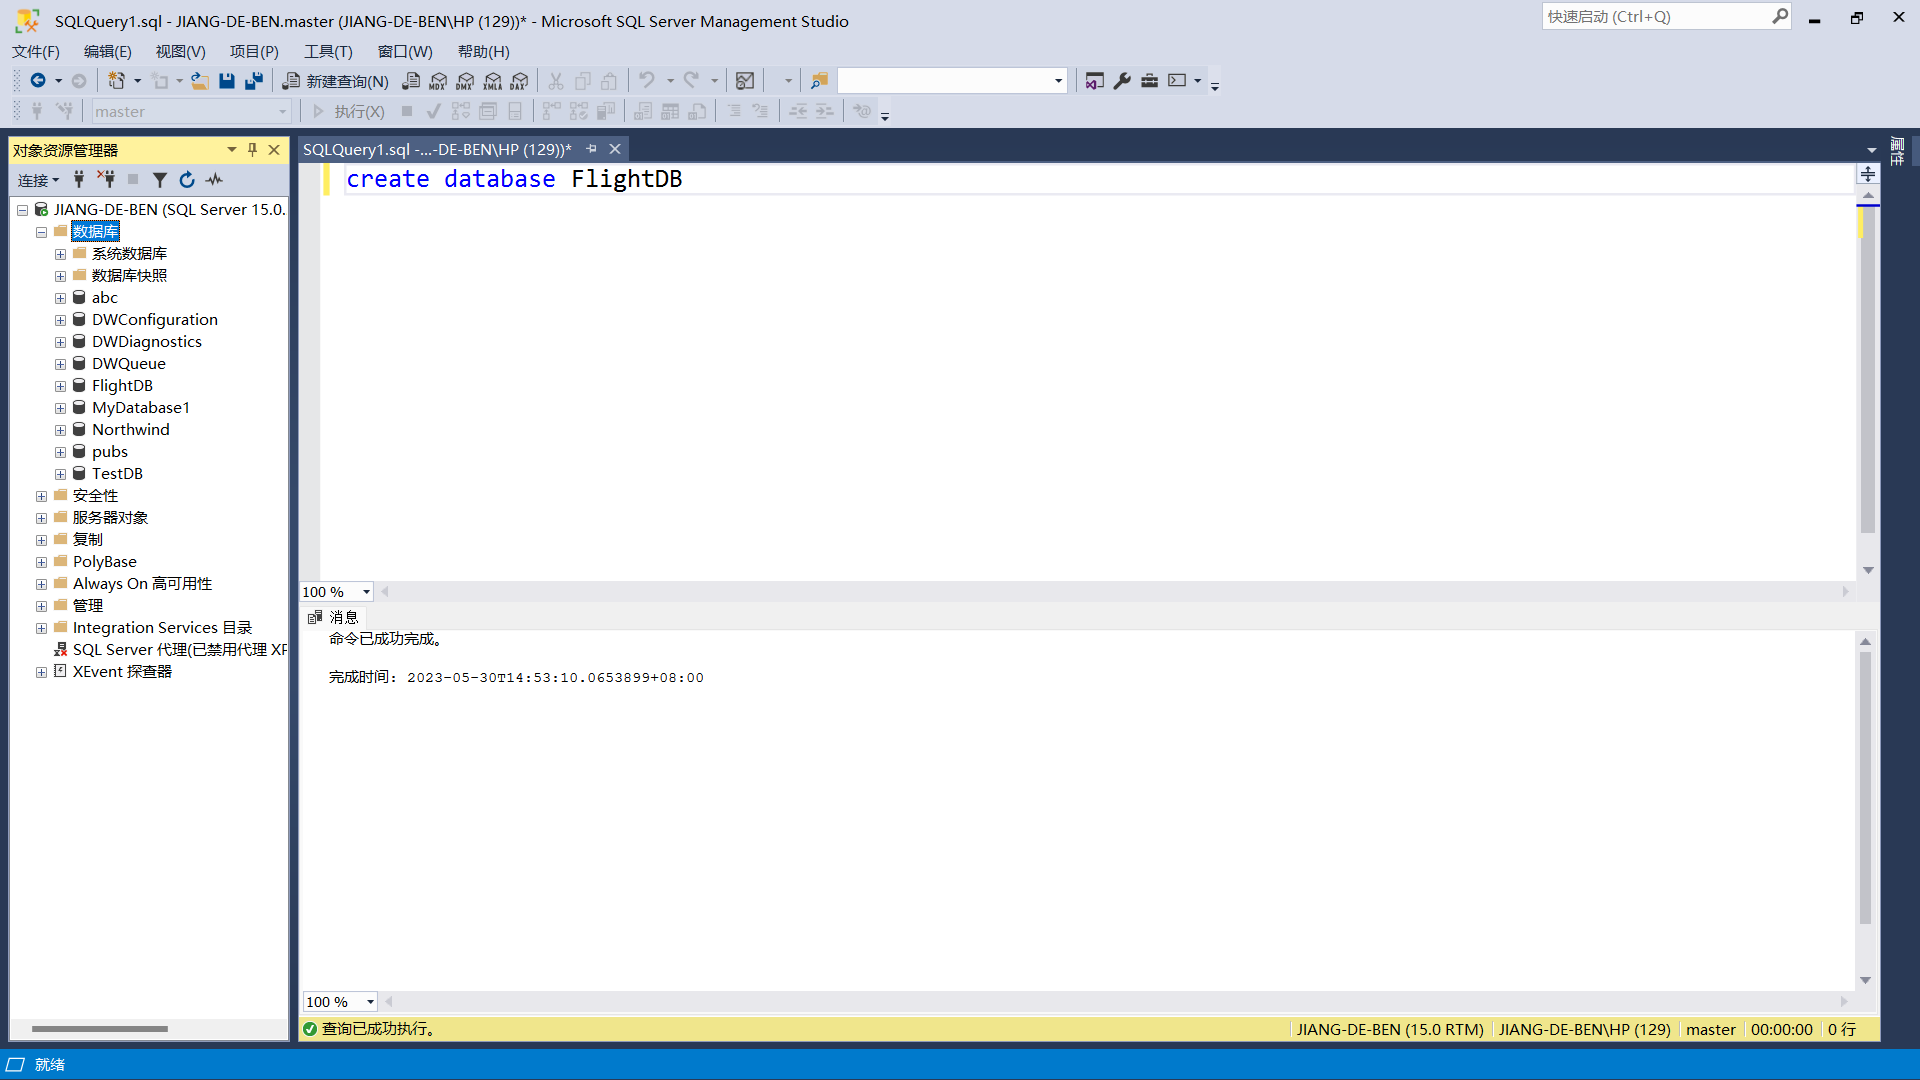
\includegraphics[width=0.8\textwidth]{img/1.png}
    \caption{DDL创建数据库}
\end{figure}

\subsection{DDL创建表}
使用DDL语句进行三张表的创建
分别实现要求中的字段,以及主码、外码、非空、默认值等约束条件

\subsubsection{航班表(hbb)}
\begin{itemize}
    \item 航班号(hbh):字符型,6位定长,主码,以CZ、CA、FM开头
    \item 始发地(sfd):字符型,可变长统一编码字符型20位长,非空
    \item 目的地(mdd):字符型,可变长统一编码字符型20位长,非空
    \item 原价(YJ):整型,非空,必须>=0
\end{itemize}

具体实现语句如下
\begin{lstlisting}[title=DDL创建航班表,frame=shadowbox]
    create table hbb
(
hbh char(6) primary key check(hbh like 'CZ%' or hbh like 'CA%' or hbh like'FM%'),
sfd varchar(20) not null,
mdd varchar(20) not null,
yj int not null check(yj>=0)
)
\end{lstlisting}

\subsubsection{乘客表(Ckb)}
\begin{itemize}
    \item 身份证号(sfzh):字符型,20位变长字符串,主码
    \item 姓名(xm):可变长统一编码字符型,10位长
\end{itemize}

具体实现语句如下
\begin{lstlisting}[title=DDL创建乘客表,frame=shadowbox]
    create table Ckb
    (
    sfzh varchar(20) primary key,
    xm varchar(10)
    )
\end{lstlisting}

\subsubsection{售票表(spb)}
\begin{itemize}
    \item 航班号(hbh):主码 
    \item 身份证号(sfzh):主码
    \item 起飞日期(qfrq):日期时间型,非空
    \item 售票日期(sprq):日期时间型,非空,默认值为当前时间
    \item 实价(sj):整型,非空
    \item 其中:航班号为引用航班表的外码,身份证号为引用乘客表的外码。
\end{itemize}

具体实现语句如下
\begin{lstlisting}[title=DDL创建售票表,frame=shadowbox]
    create table spb
    (
    hbh char(6) references hbb(hbh) on delete cascade,
    sfzh varchar(20) references Ckb(sfzh) on delete cascade,
    qfrq date not null,
    sprq date not null default getdate(),
    sj int not null,
    
    primary key(hbh,sfzh)
    )
\end{lstlisting}


最终在SQL Server Management Studio中的效果如下
\begin{figure}[htbp]
    \centering
    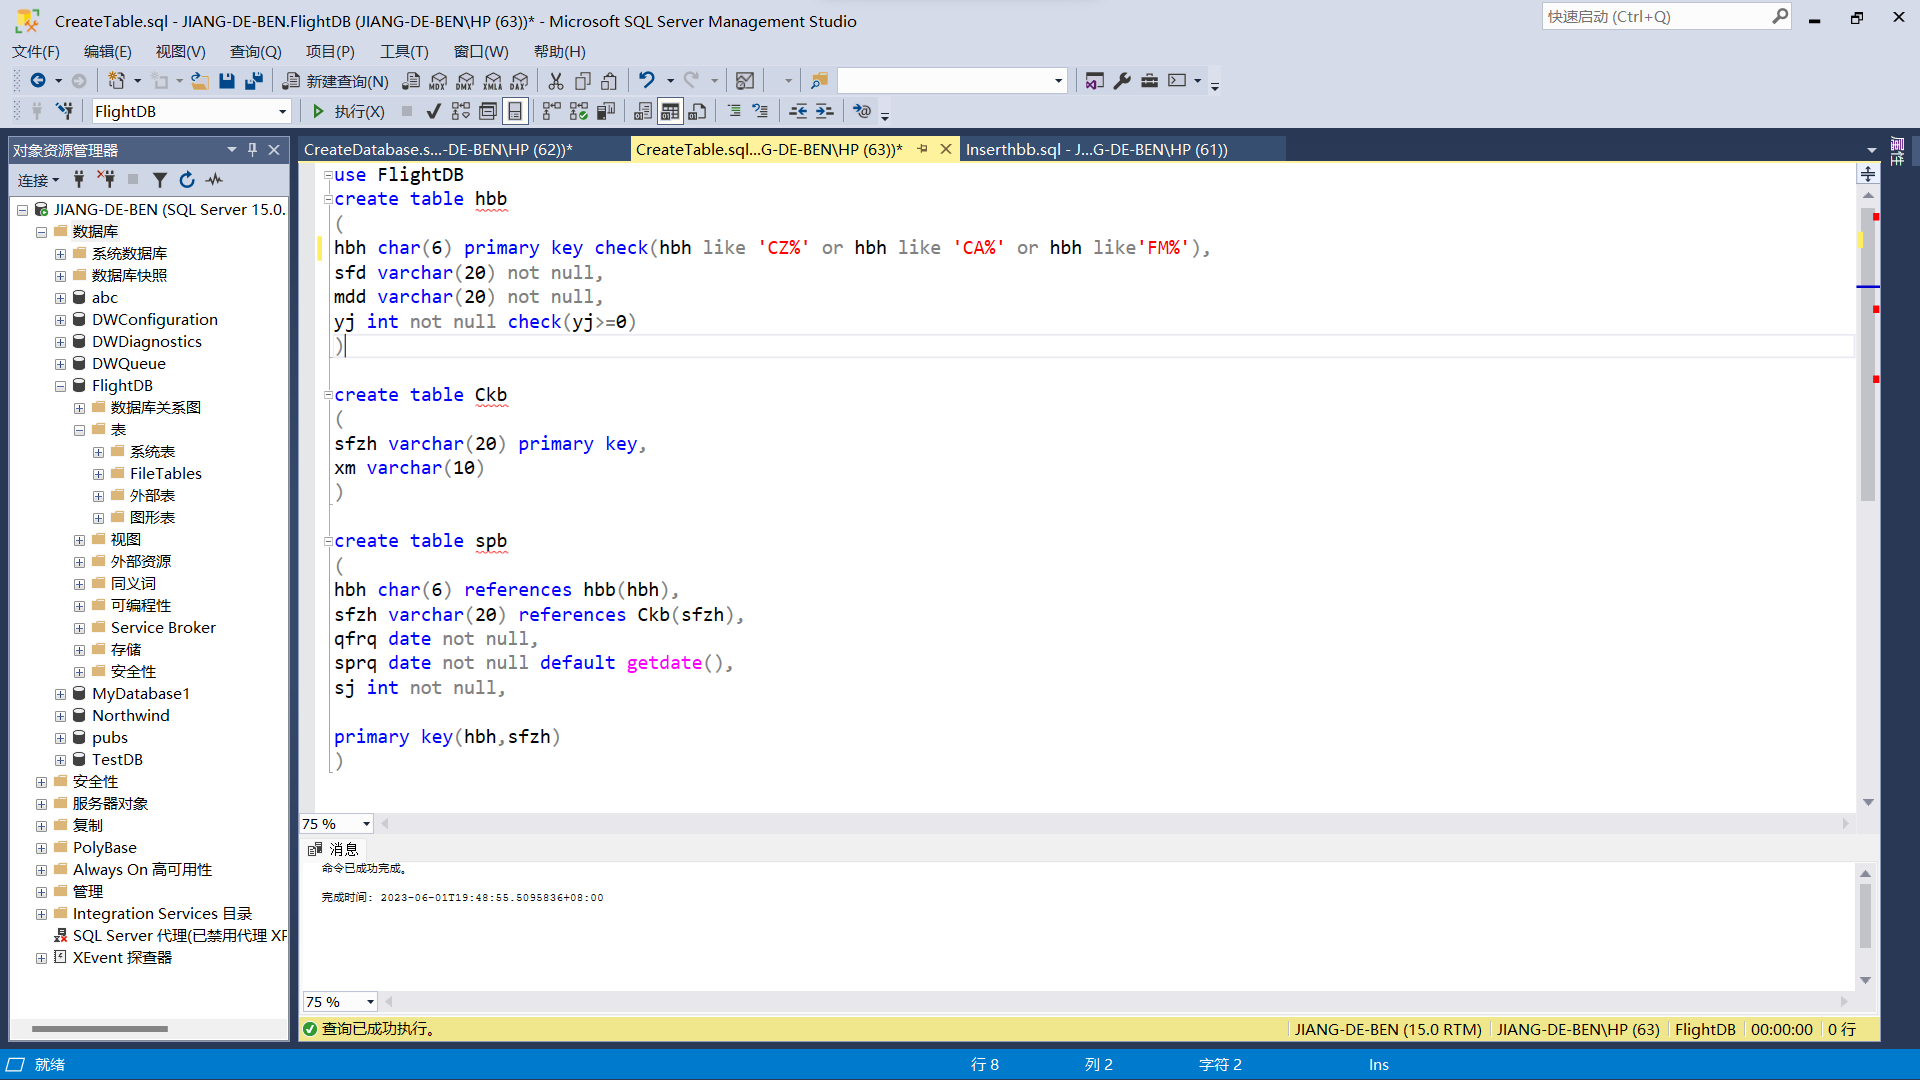
\includegraphics[width=0.8\textwidth]{img/2.png}
    \caption{DDL创建表}
\end{figure}

\subsection{DML插入hbb数据}
使用DML语句在hbb表中插入数据
\begin{lstlisting}[title=DML插入hbb数据,frame=shadowbox]
    insert into hbb values
    ('CZ1301','北京','上海',1200),
    ('CZ1209','南京','昆明',1300),
    ('CZ1502','上海','北京',1200),
    ('CA1130','成都','北京',1800),
    ('CA1230','拉萨','广州',1500),
    ('CA1401','广州','南京',1600)
\end{lstlisting}

实现效果如下
\begin{figure}[htbp]
	\centering
	\begin{minipage}{0.7\linewidth}
		\centering
		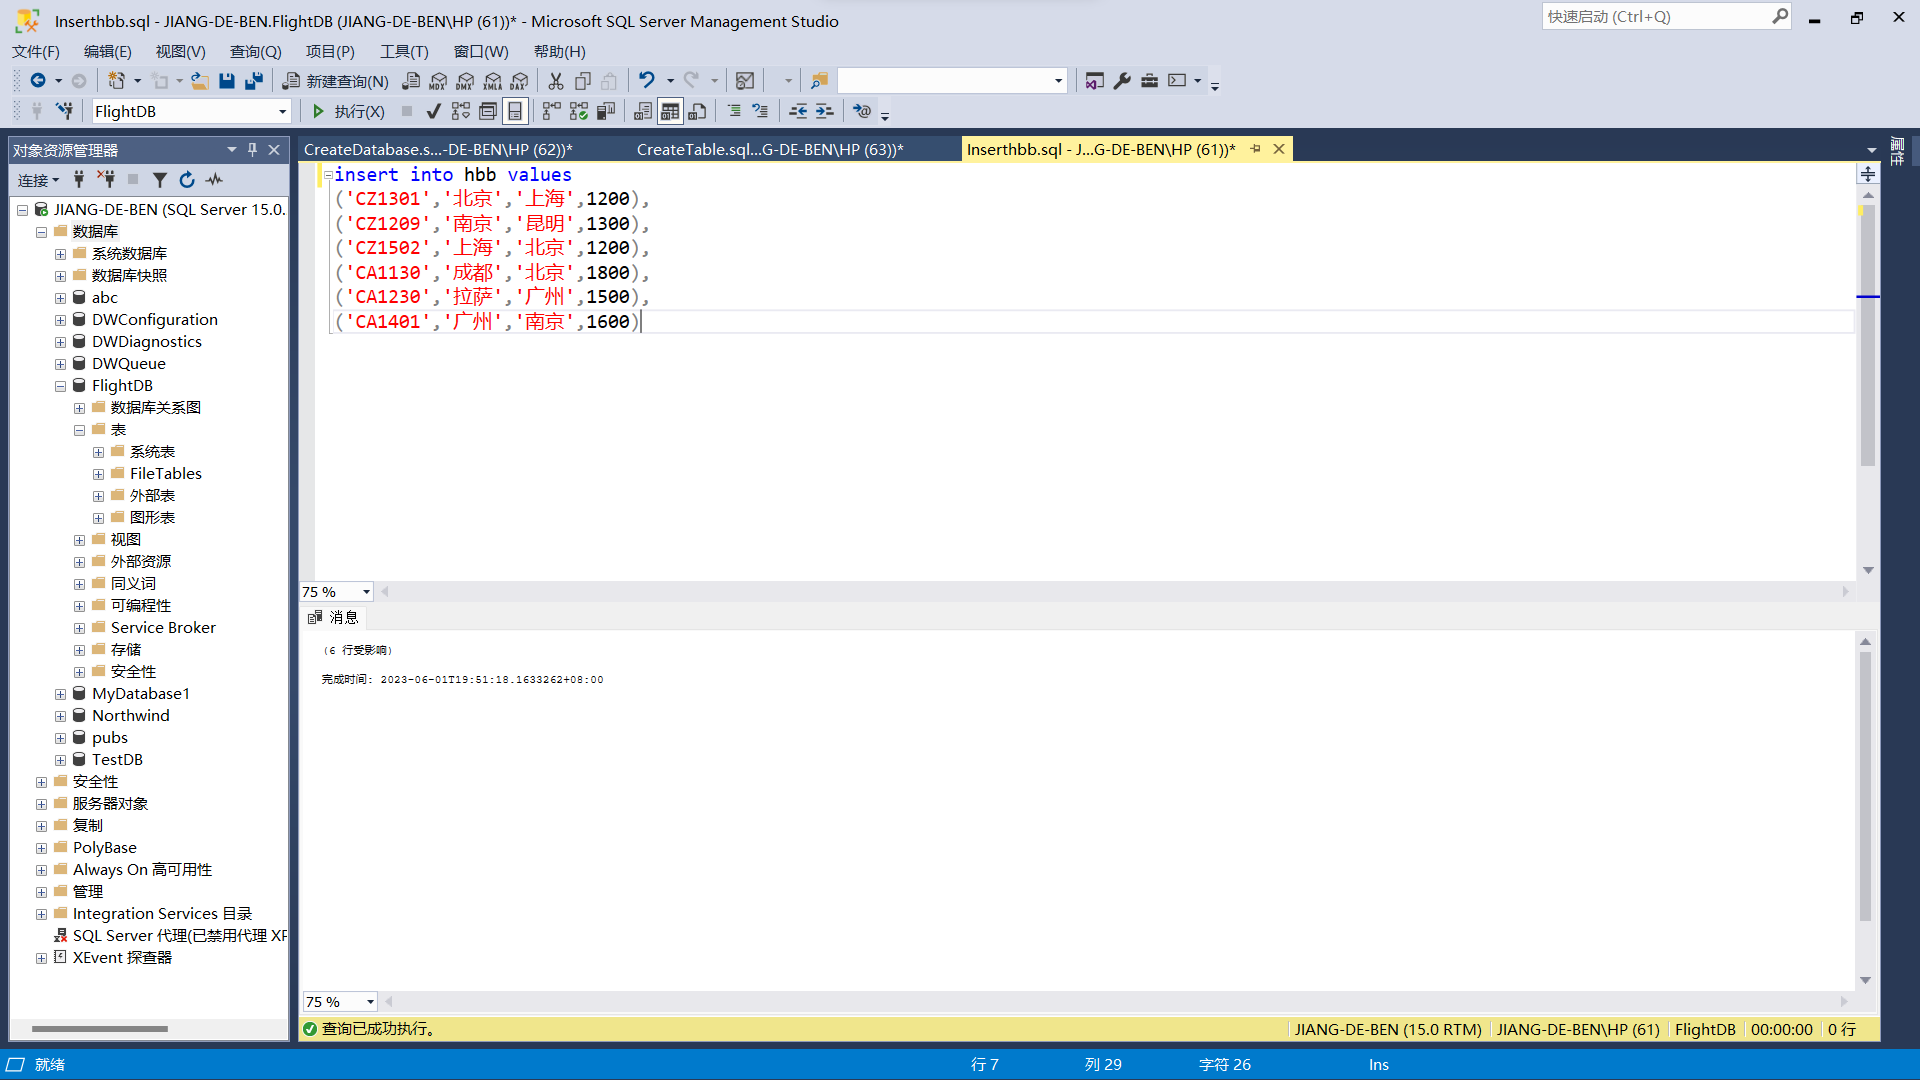
\includegraphics[width=0.9\linewidth]{img/3.png}
	\end{minipage}
	\begin{minipage}{0.7\linewidth}
		\centering
		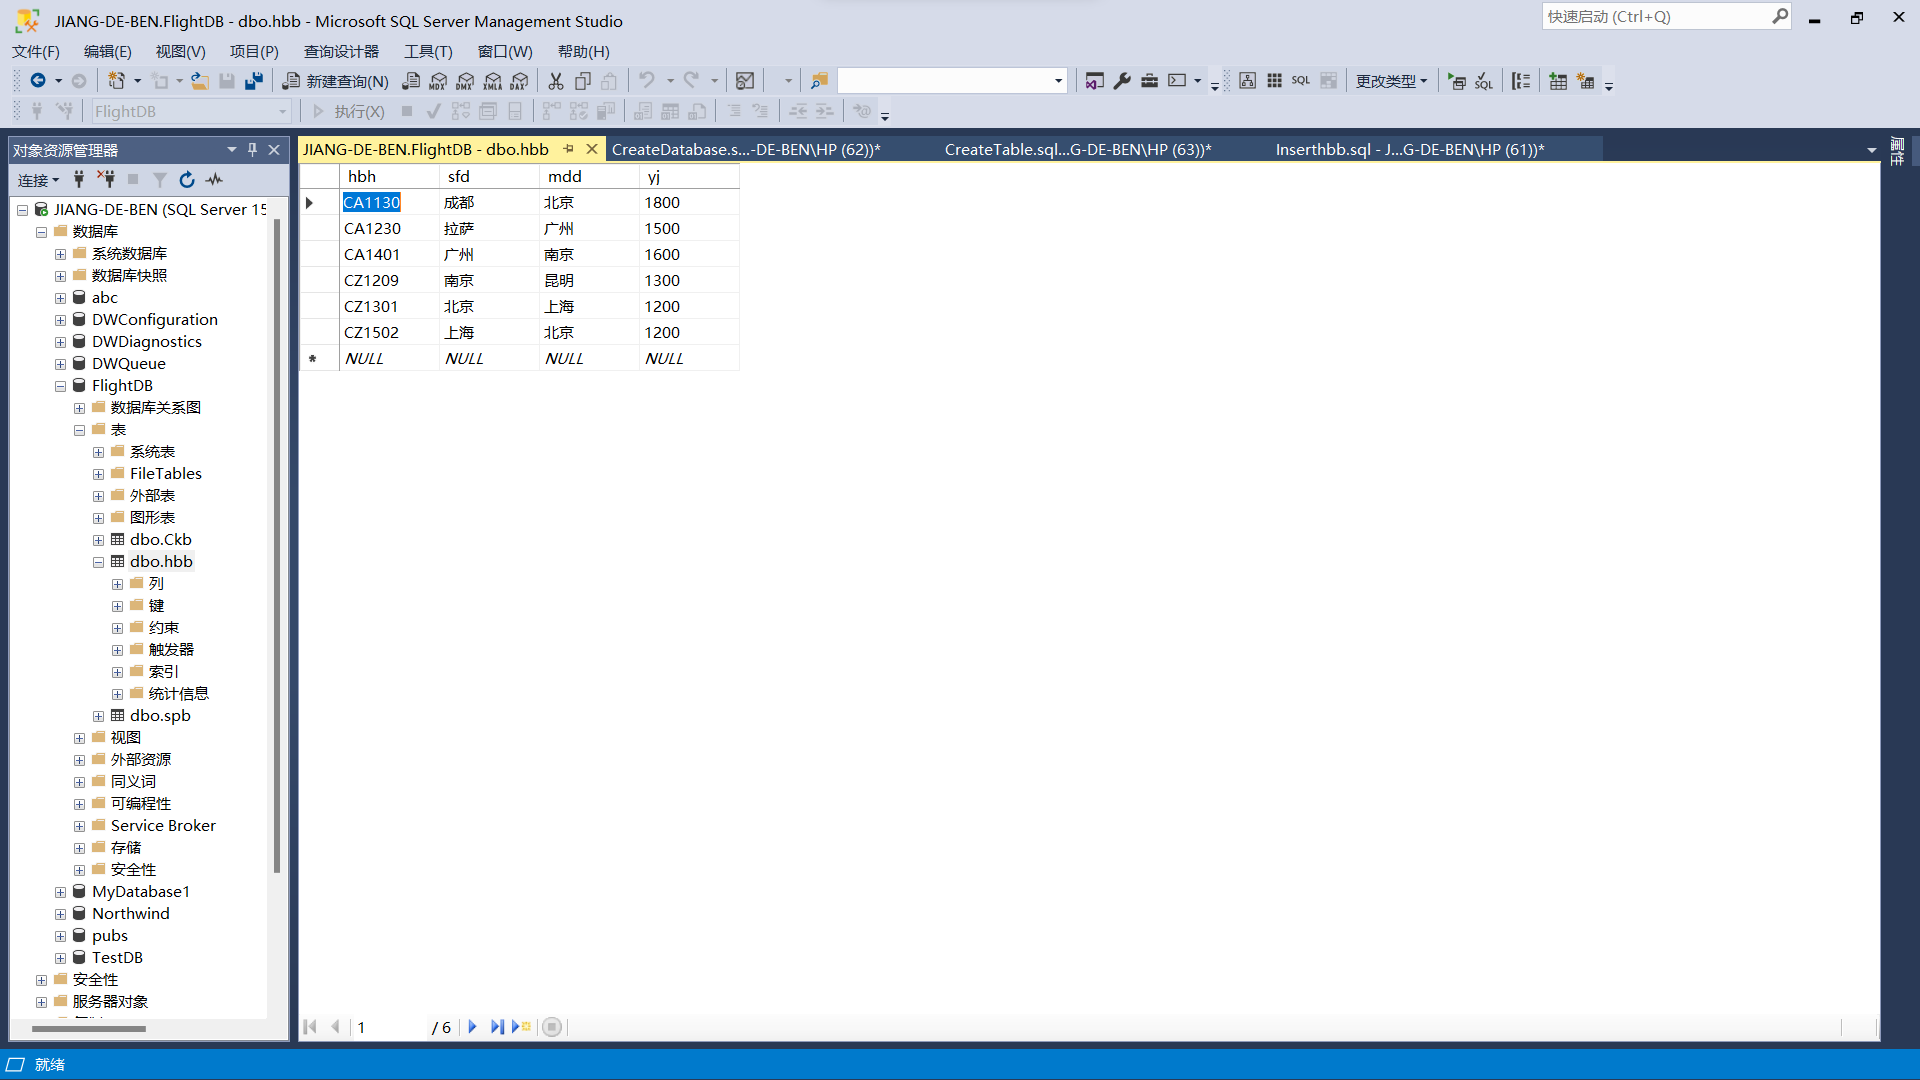
\includegraphics[width=0.9\linewidth]{img/4.png}
	\end{minipage}
    \caption{DML插入hbb数据}
\end{figure}

\subsection{完整备份}
使用SQL Server的备份功能,对数据库进行一次完整备份,备份名为BackupFull

实现代码如下
\begin{lstlisting}[title=完整备份,frame=shadowbox]
    backup database FlightDB
    to disk='E:\sql\MSSQL15.MSSQLSERVER\MSSQL\Backup\BackupFull.bak'
    with format,
    name='BackupFull',
    description='数据库FlightDB的备份'
\end{lstlisting}

实现效果如下
\begin{figure}[htbp]
	\centering
	\begin{minipage}{0.5\linewidth}
		\centering
		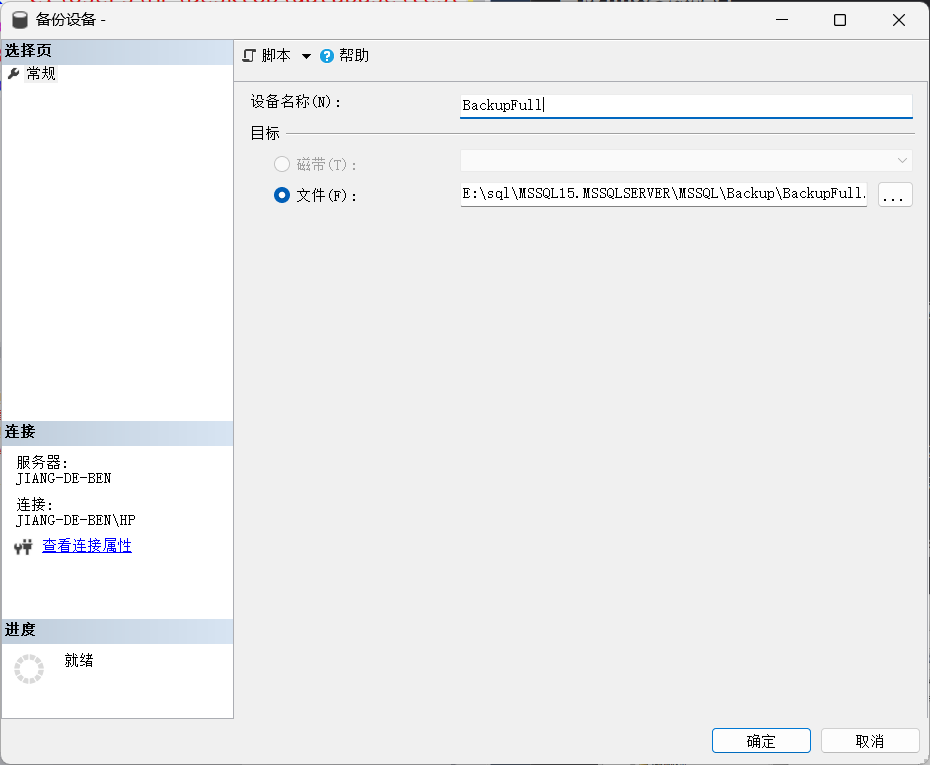
\includegraphics[width=0.9\linewidth]{img/5.png}
	\end{minipage}
	\begin{minipage}{0.5\linewidth}
		\centering
		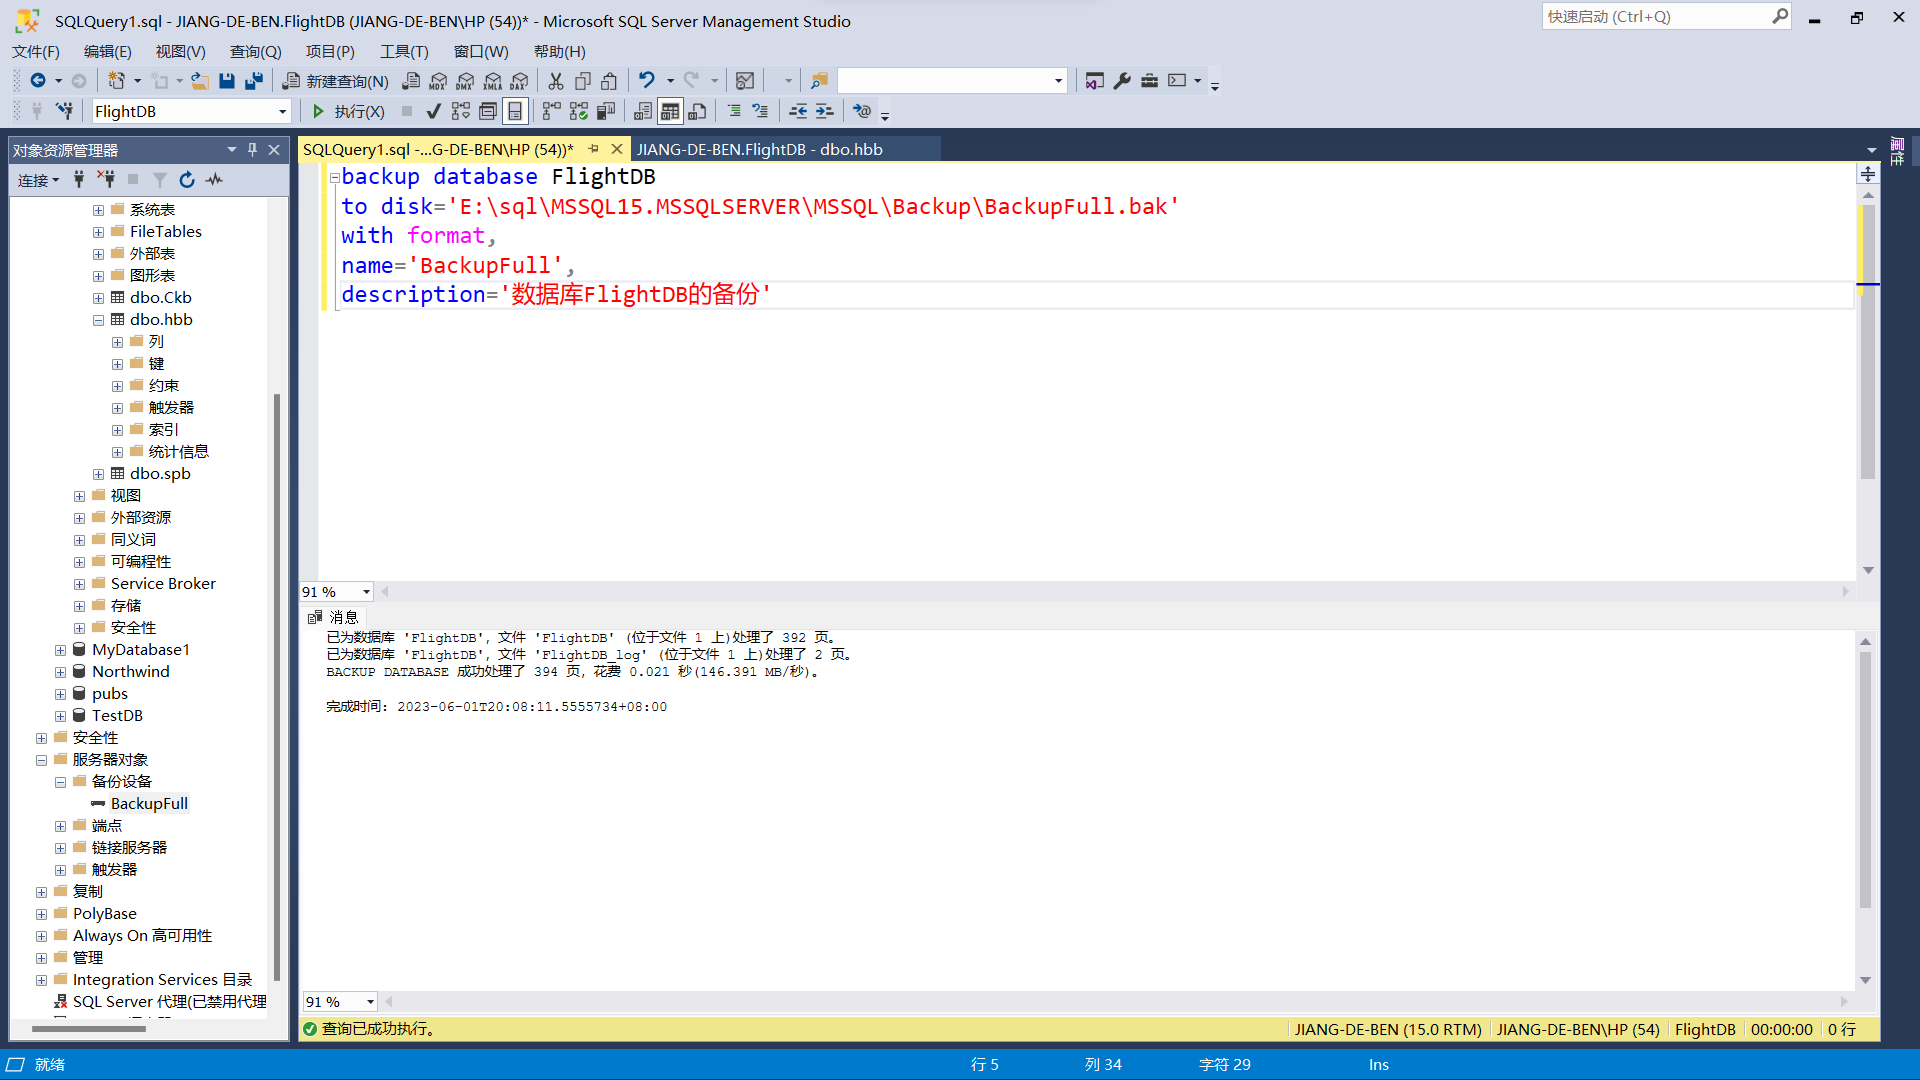
\includegraphics[width=0.9\linewidth]{img/6.png}
	\end{minipage}
    \caption{完整备份}
\end{figure}

\subsection{DML插入Ckb和spb数据}
使用DML语句在Ckb表和spb表中插入数据
\begin{lstlisting}[title=DML插入Ckb和spb数据,frame=shadowbox]
    insert into Ckb values
('91201','王曼'),
('91202','张飞'),
('91203','刘羽蕴'),
('91204','王若雨'),
('91205','张蕊')

    insert into spb values
('CZ1301','91201','2001-12-20','2001-11-20',900),
('CZ1209','91202','2001-12-20','2001-11-20',800),
('CZ1502','91201','2002-5-8','2002-5-2',1000),
('CA1230','91201','2001-12-5','2001-12-4',1100),
('CA1401','91202','2002-4-5','2002-4-4',1200),
('CZ1301','91203','2001-12-20','2001-11-20',900),
('CZ1209','91204','2001-12-20','2001-11-20',800),
('CZ1502','91205','2002-5-8','2002-5-2',1000)
\end{lstlisting}

实现效果如下

\begin{figure}[htbp]
    \centering
    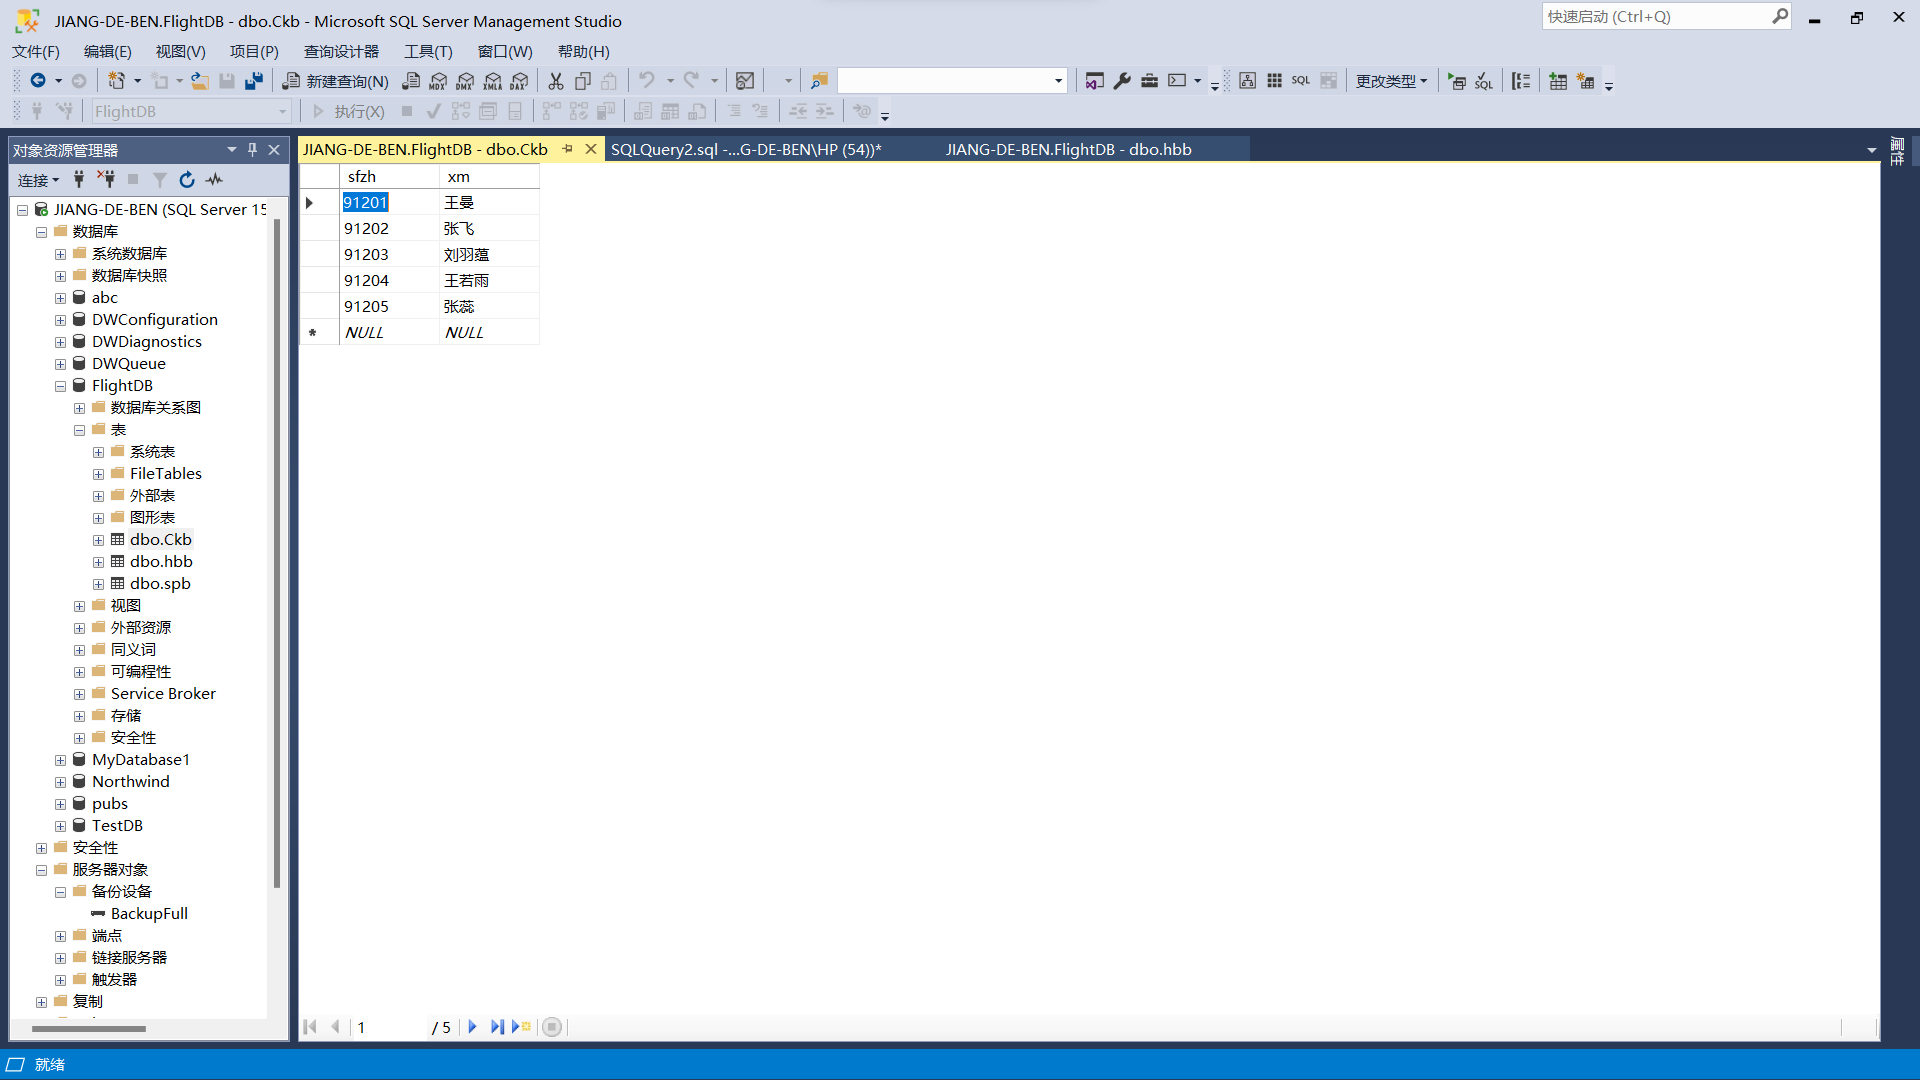
\includegraphics[width=0.7\textwidth]{img/7.png}
    \caption{DML插入Ckb}
\end{figure}

\begin{figure}[htbp]
    \centering
    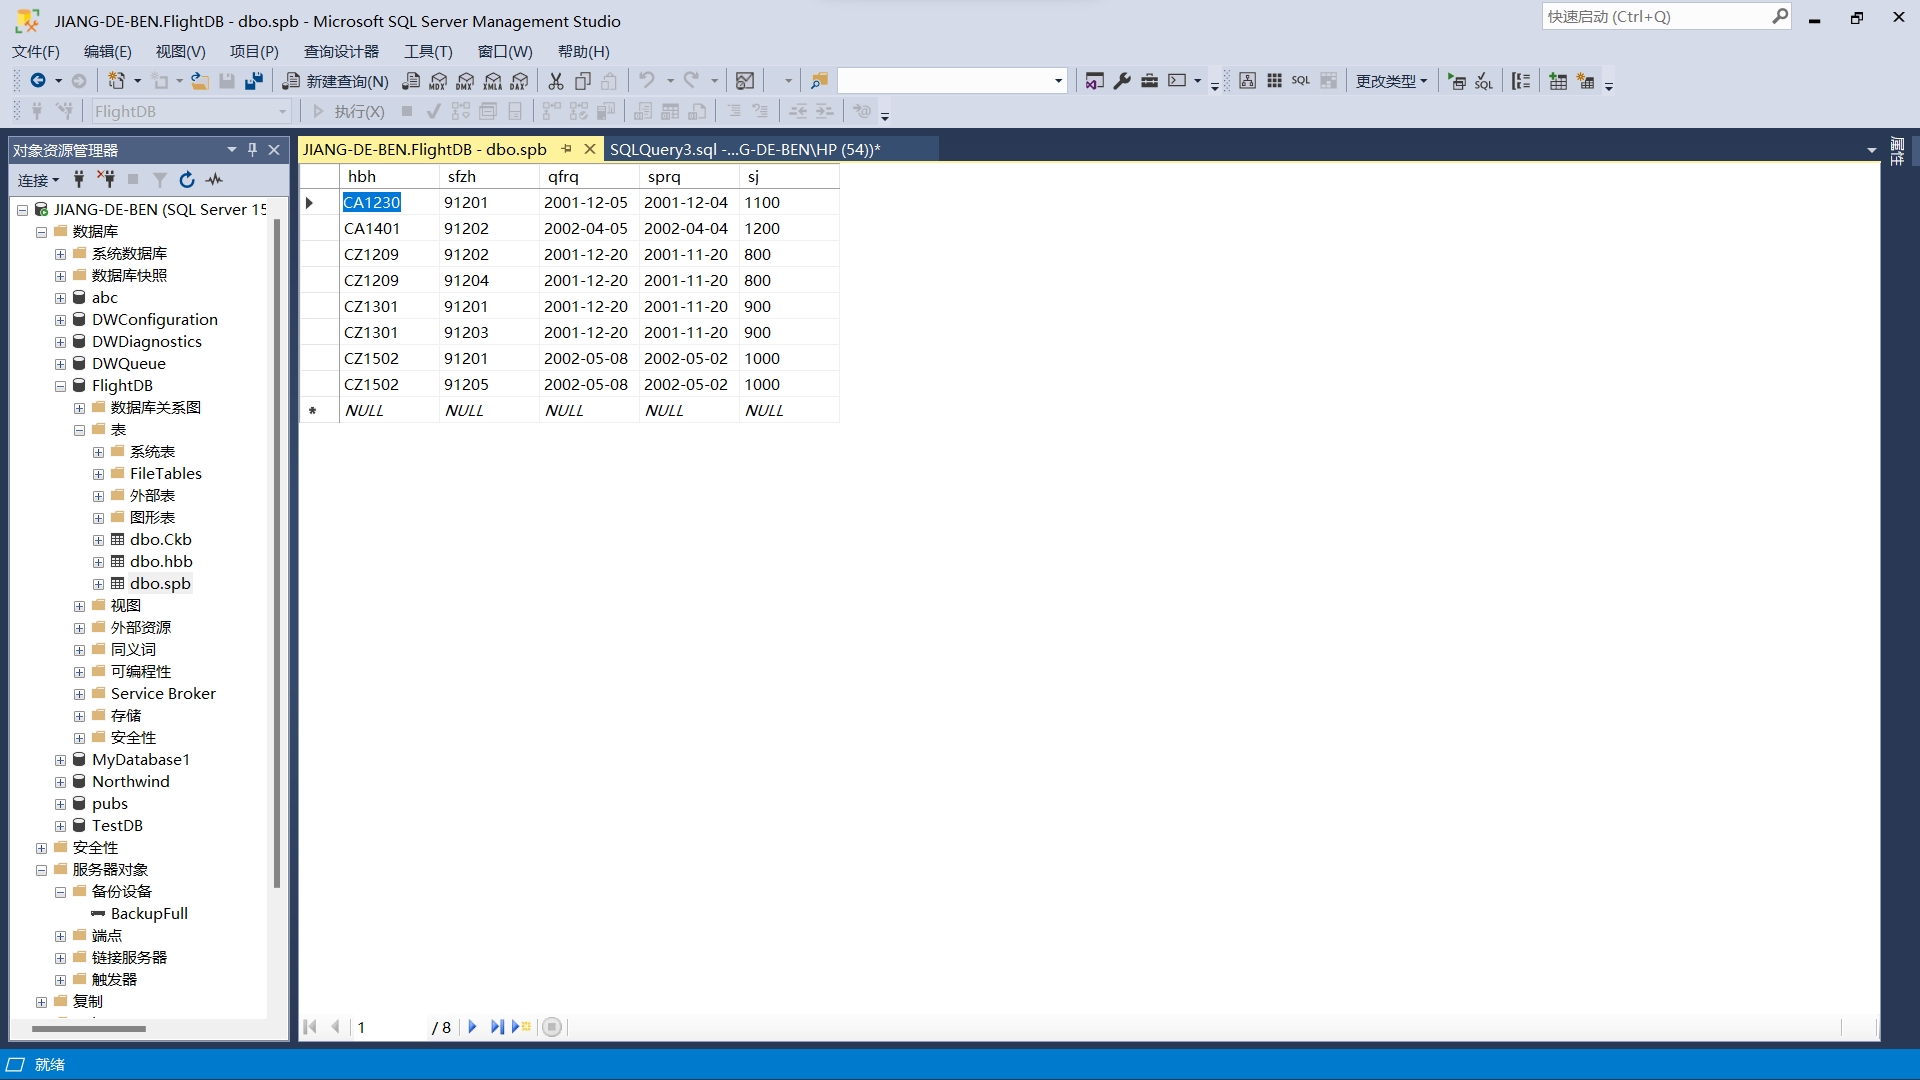
\includegraphics[width=0.7\textwidth]{img/8.png}
    \caption{DML插入spb}
\end{figure}

\subsection{差异备份}
使用SQL Server的备份功能,对数据库进行一次差异备份,备份名为BackupAdd1

在这一部分中使用了GUI界面进行操作,实现效果如下
\begin{figure}[htbp]
    \centering
    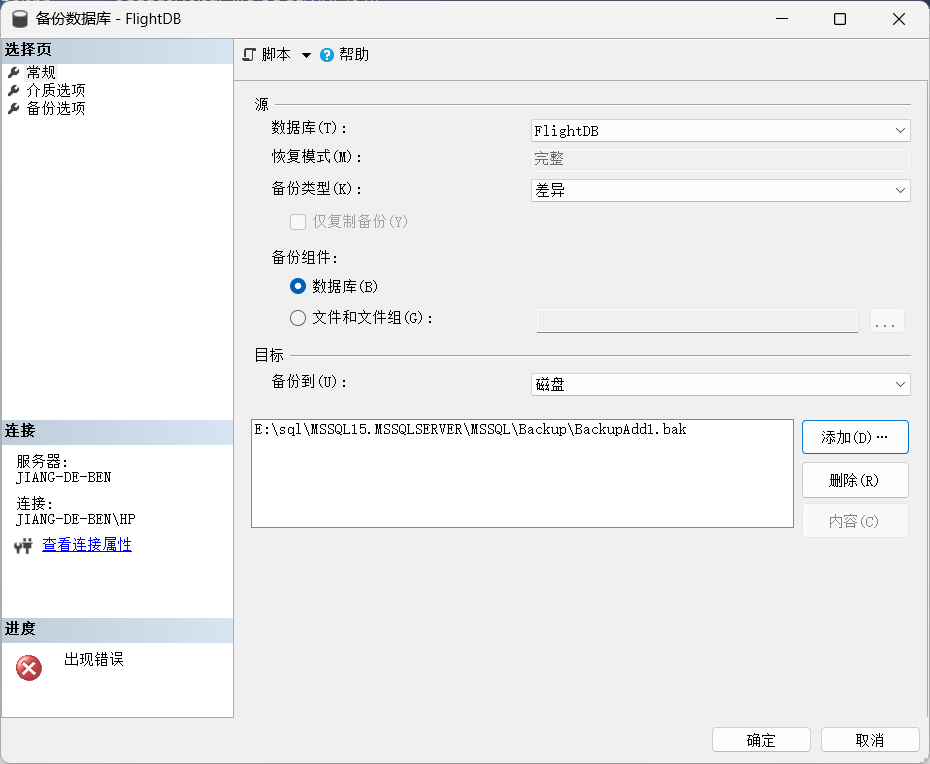
\includegraphics[width=0.56\textwidth]{img/9.png}
    \caption{差异备份}
\end{figure}

\subsection{DML更新hbb数据}
使用DML语句将所有目的地是北京的航班的原价提高10\%,实现代码如下
\begin{lstlisting}[title=DML更新hbb数据,frame=shadowbox]
    select * from hbb
    where mdd='北京'
    
    update hbb
    set yj=yj*1.1
    where mdd='北京'
    
    select * from hbb
    where mdd='北京'    
\end{lstlisting}

更改前后的票价展示如下
\begin{figure}[htbp]
    \centering
    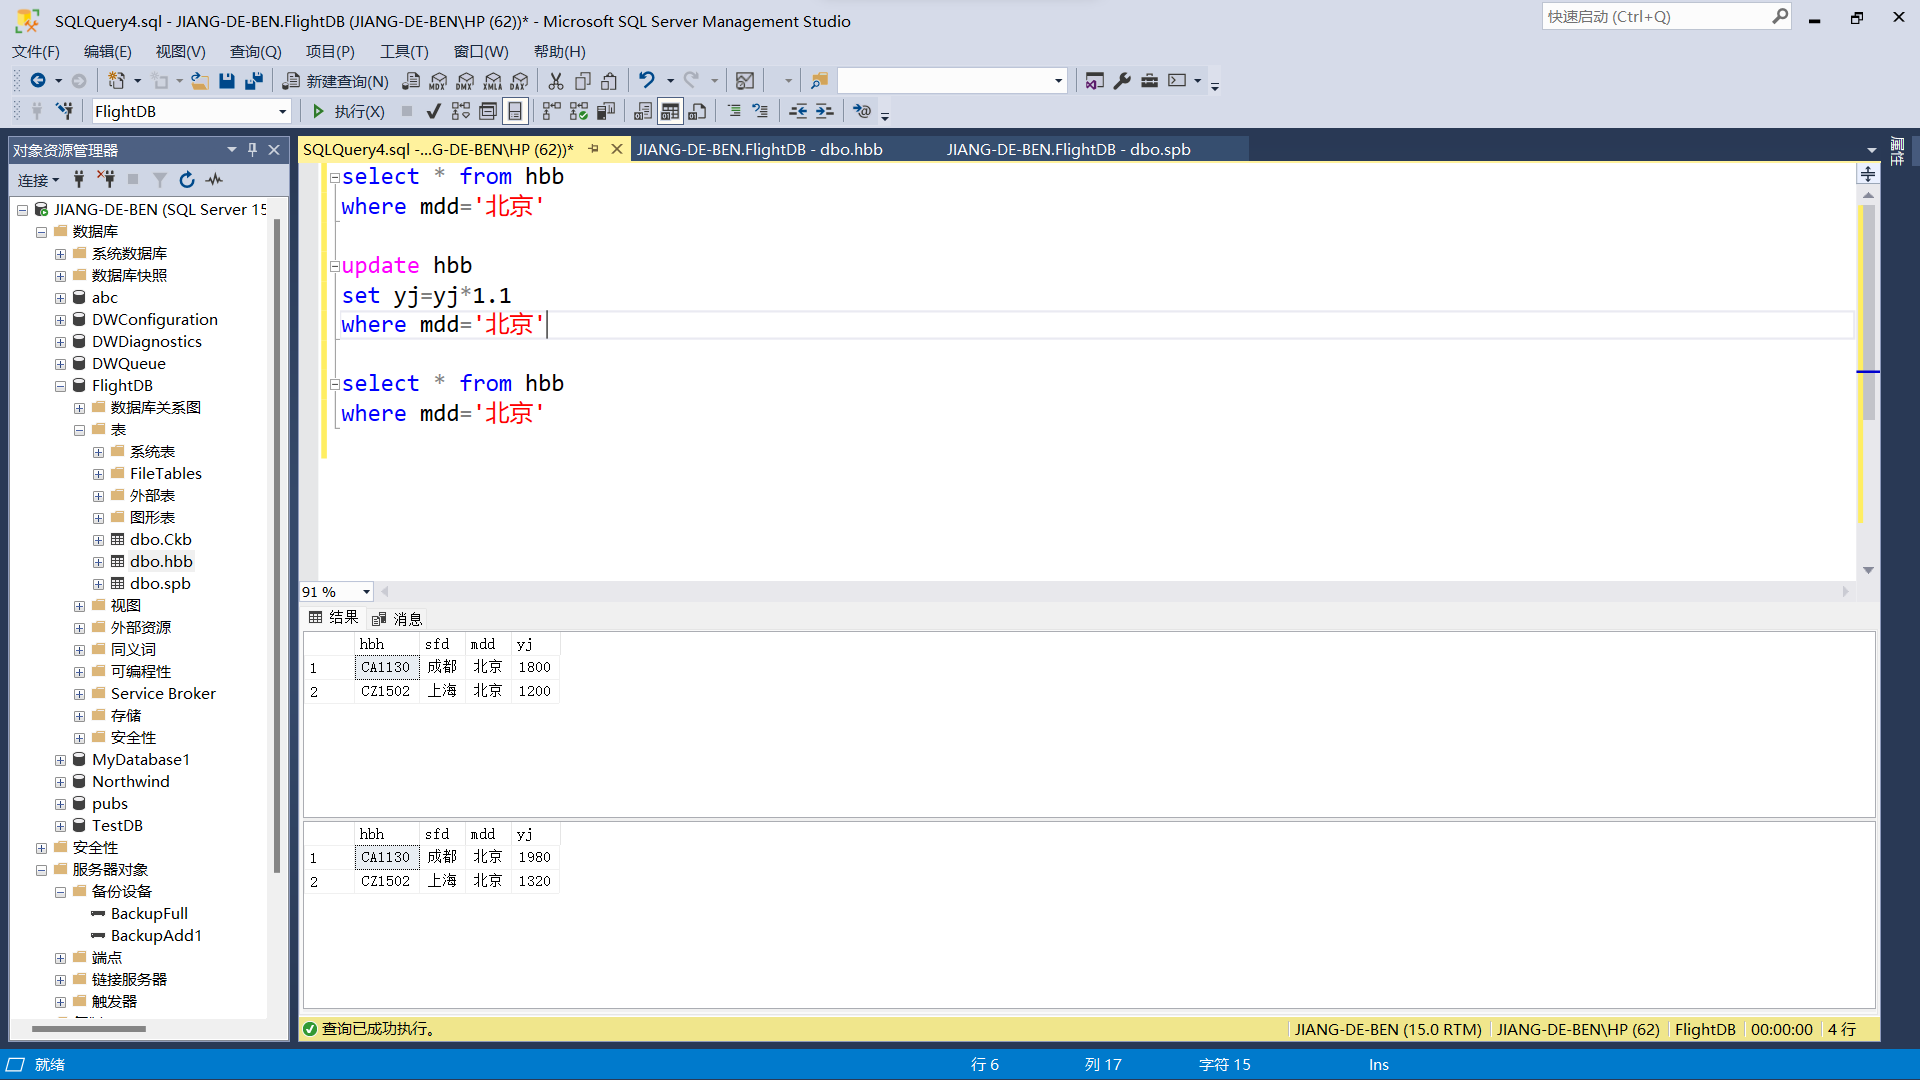
\includegraphics[width=0.8\textwidth]{img/10.png}
    \caption{DML更新hbb数据}
\end{figure}

\subsection{DML删除Ckb数据}
使用DML语句将“张飞”乘客删除,注意同时删除售票记录和乘客基本信息,由于在创建表的时候使用了外码约束,所以在删除乘客信息的时候会自动删除售票信息

实现代码如下
\begin{lstlisting}[title=DML删除Ckb数据,frame=shadowbox]
    select * from Ckb
    
    delete from Ckb
    where xm='张飞'
    
    select * from Ckb
\end{lstlisting}

实现效果如下
\begin{figure}[htbp]
    \centering
	\begin{minipage}{0.6\linewidth}
		\centering
		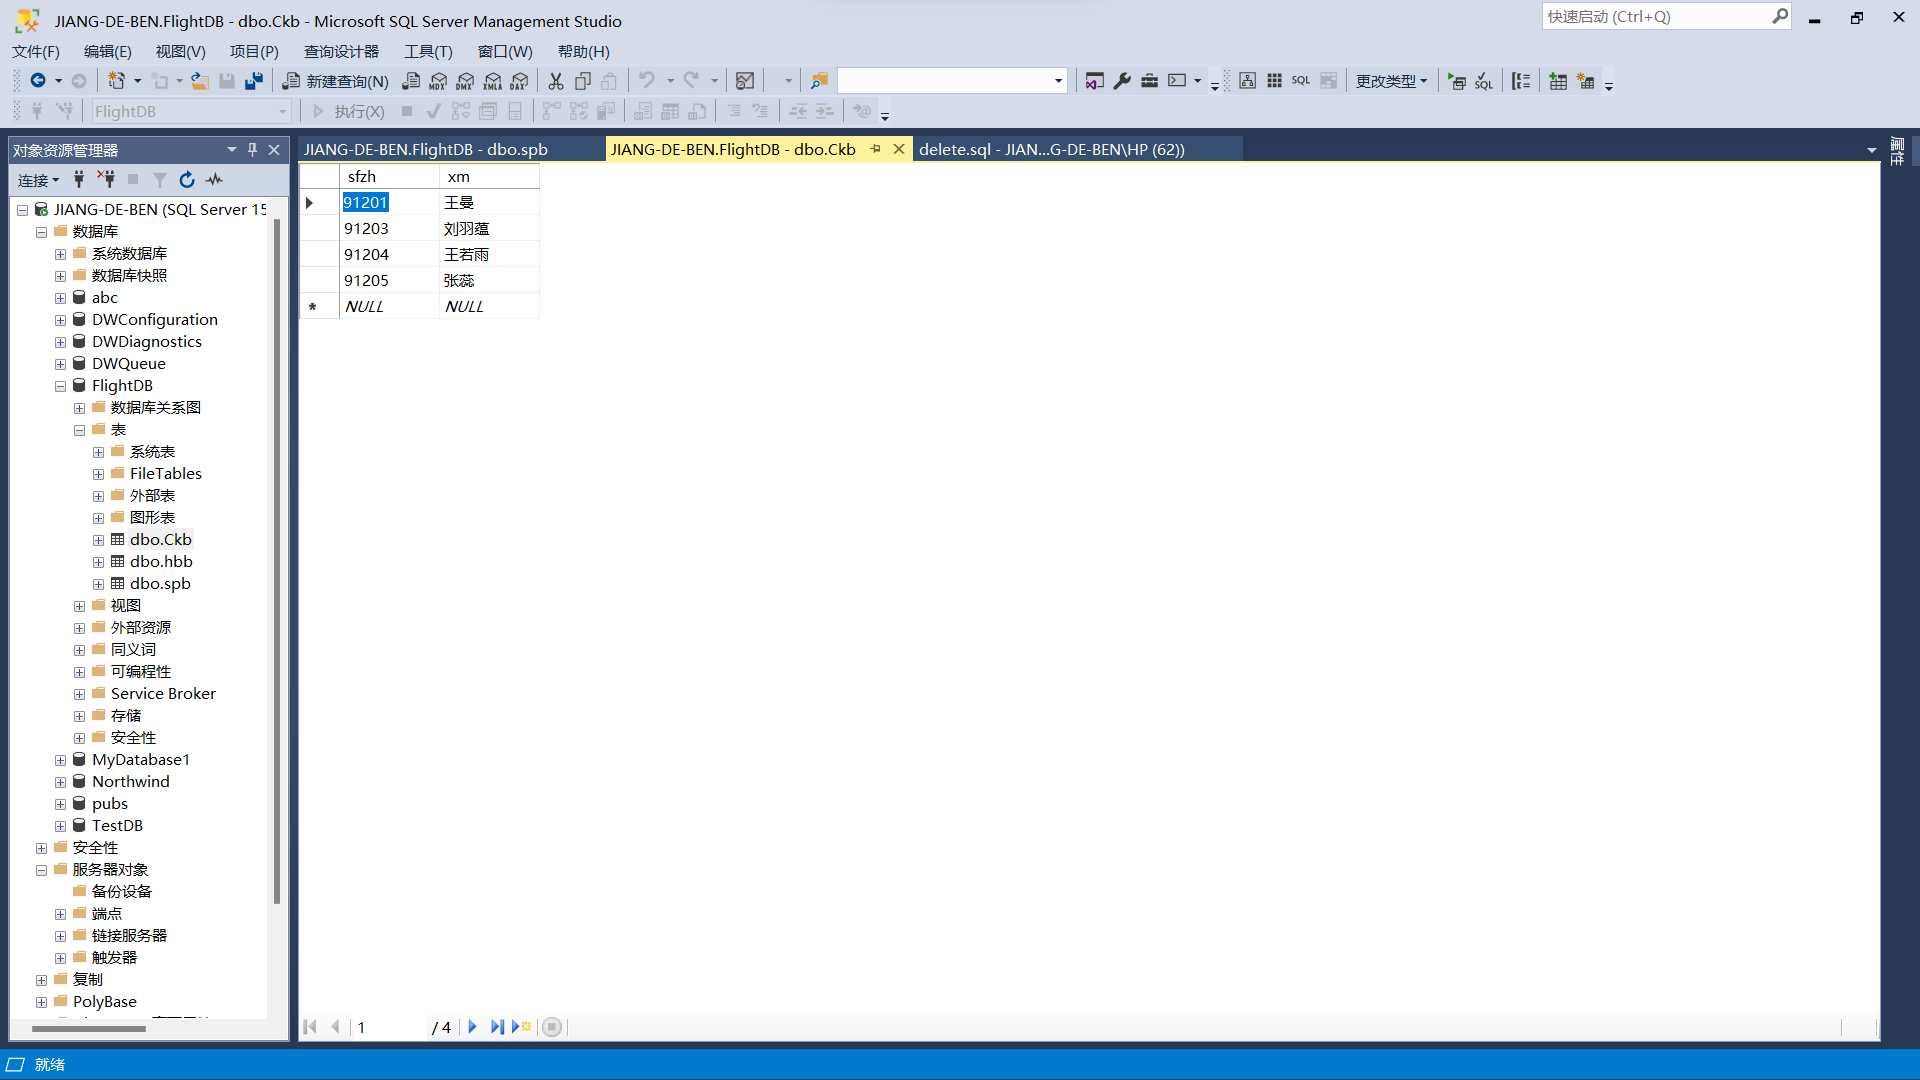
\includegraphics[width=0.9\linewidth]{img/11.png}
	\end{minipage}
	\begin{minipage}{0.6\linewidth}
		\centering
		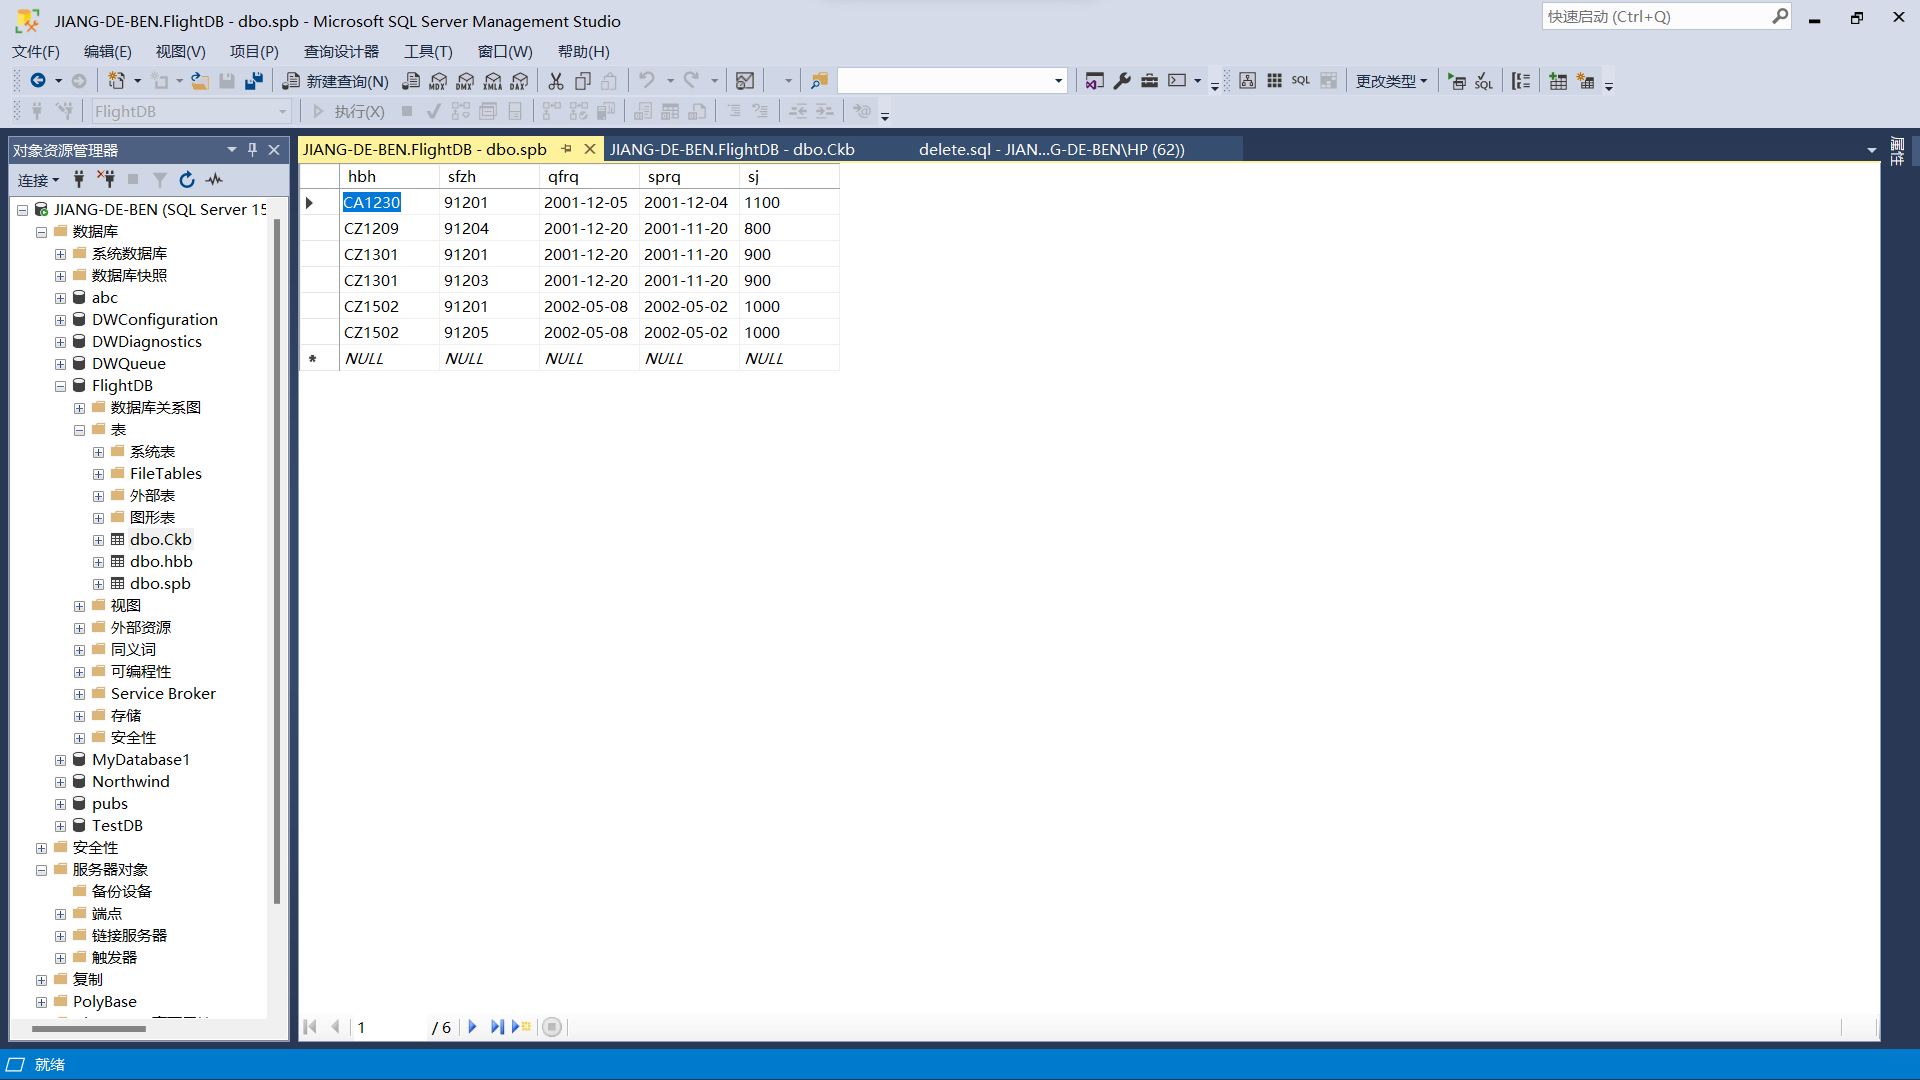
\includegraphics[width=0.9\linewidth]{img/12.png}
	\end{minipage}
    \caption{DML删除Ckb数据}
\end{figure}

\subsection{还原数据库}
使用SQL Server的还原功能,还原到上一次差异备份的BackupAdd1处

在这一部分中使用了GUI界面进行操作,实现效果如下

\begin{figure}[htbp]
    \centering
	\begin{minipage}{0.8\linewidth}
		\centering
		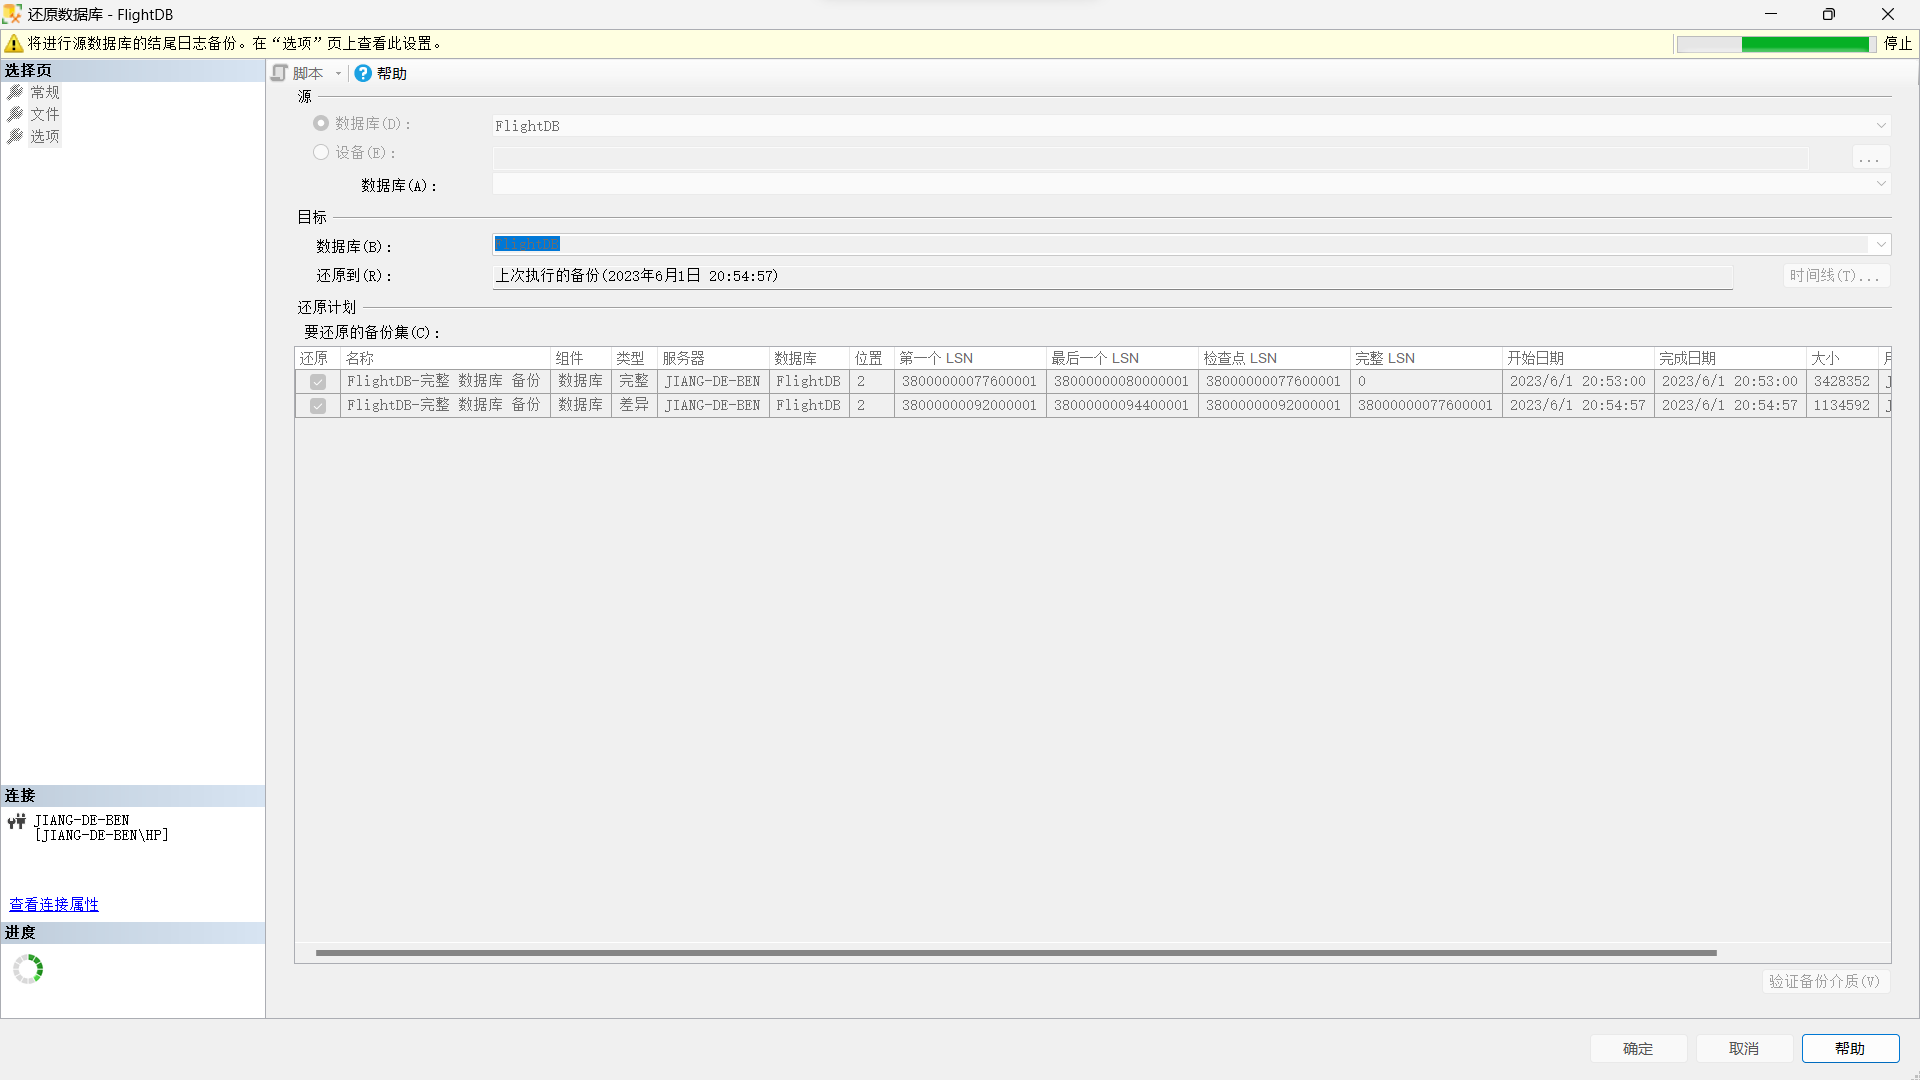
\includegraphics[width=0.9\linewidth]{img/13.png}
	\end{minipage}
	\begin{minipage}{0.8\linewidth}
		\centering
		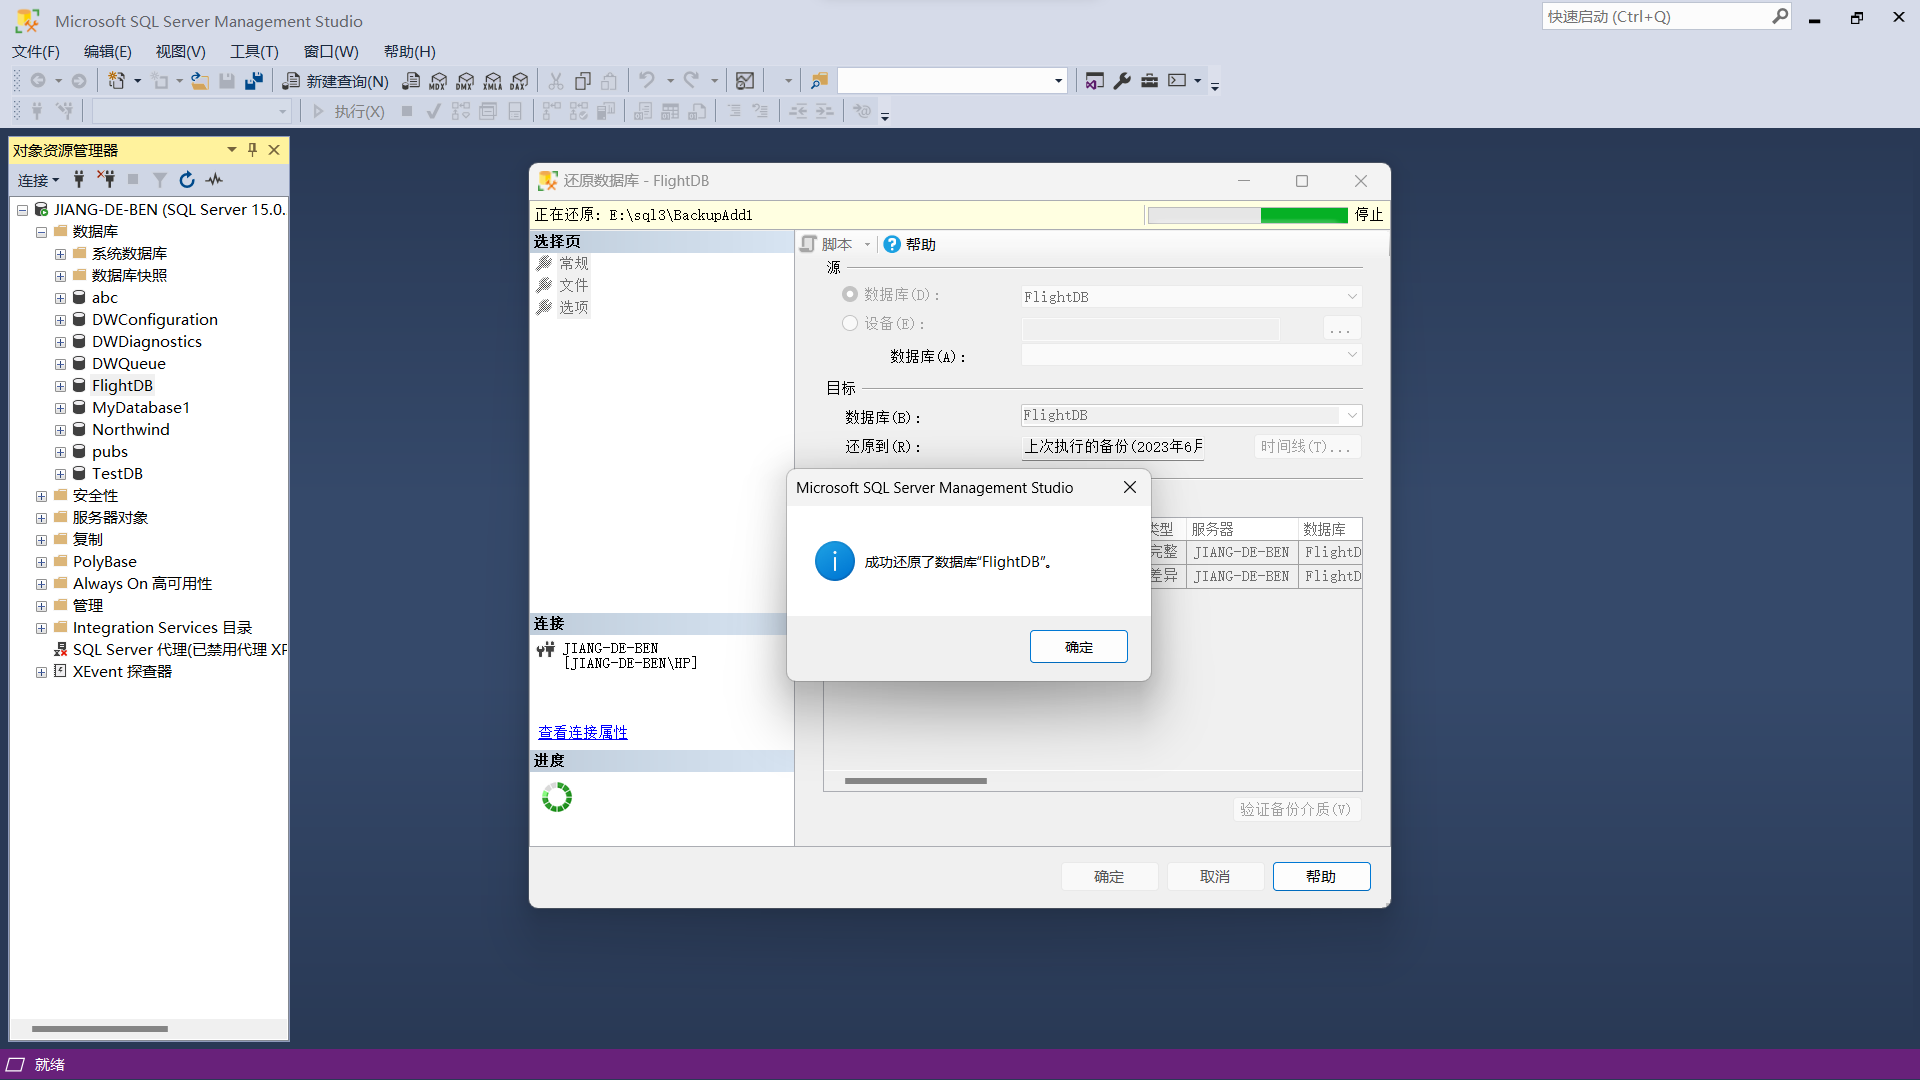
\includegraphics[width=0.9\linewidth]{img/14.png}
	\end{minipage}
    \caption{还原数据库}
\end{figure}

\subsection{创建用户}
在SQL Server中创建一个用户FlightUser,设置FlightUser用户对三张表都有查询权,但是该用户不能对乘客表和航班表进行增加、删除和修改记录,该用户对售票表能增加、删除和修改记录。然后用FlightUser登陆SQL Server,对如上权限设置进行验证

实现代码如下
\begin{lstlisting}[title=创建用户,frame=shadowbox]
    exec sp_addlogin 'FlightUser','123','FlightDB'
    grant insert,select,update,delete on spb to public
    grant select on hbb to public
    grant select on ckb to public
\end{lstlisting}

使用FlightUser登陆SQL Server,对如上权限设置进行验证,实现效果如下
\begin{figure}[htbp]
    \centering
    \begin{minipage}{0.8\linewidth}
        \centering
        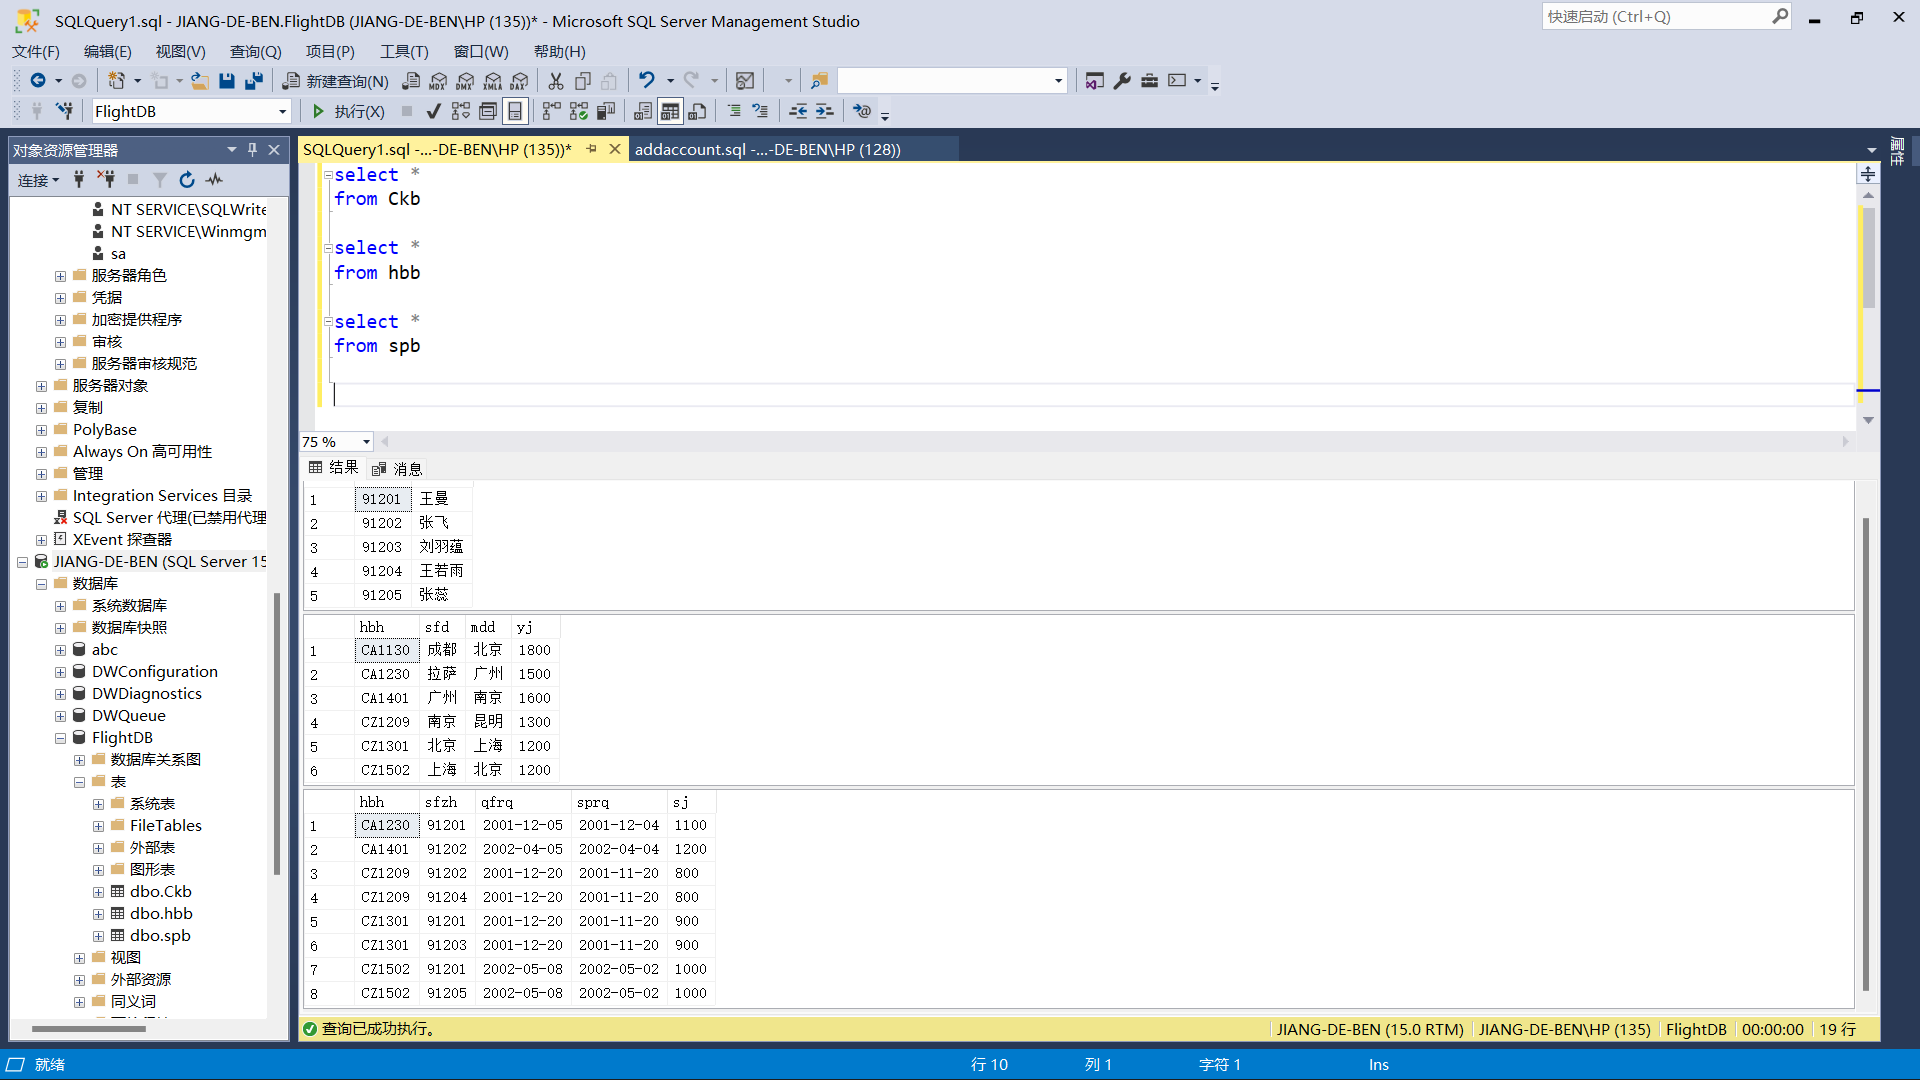
\includegraphics[width=0.9\linewidth]{img/15.png}
    \end{minipage}
    \begin{minipage}{0.8\linewidth}
        \centering
        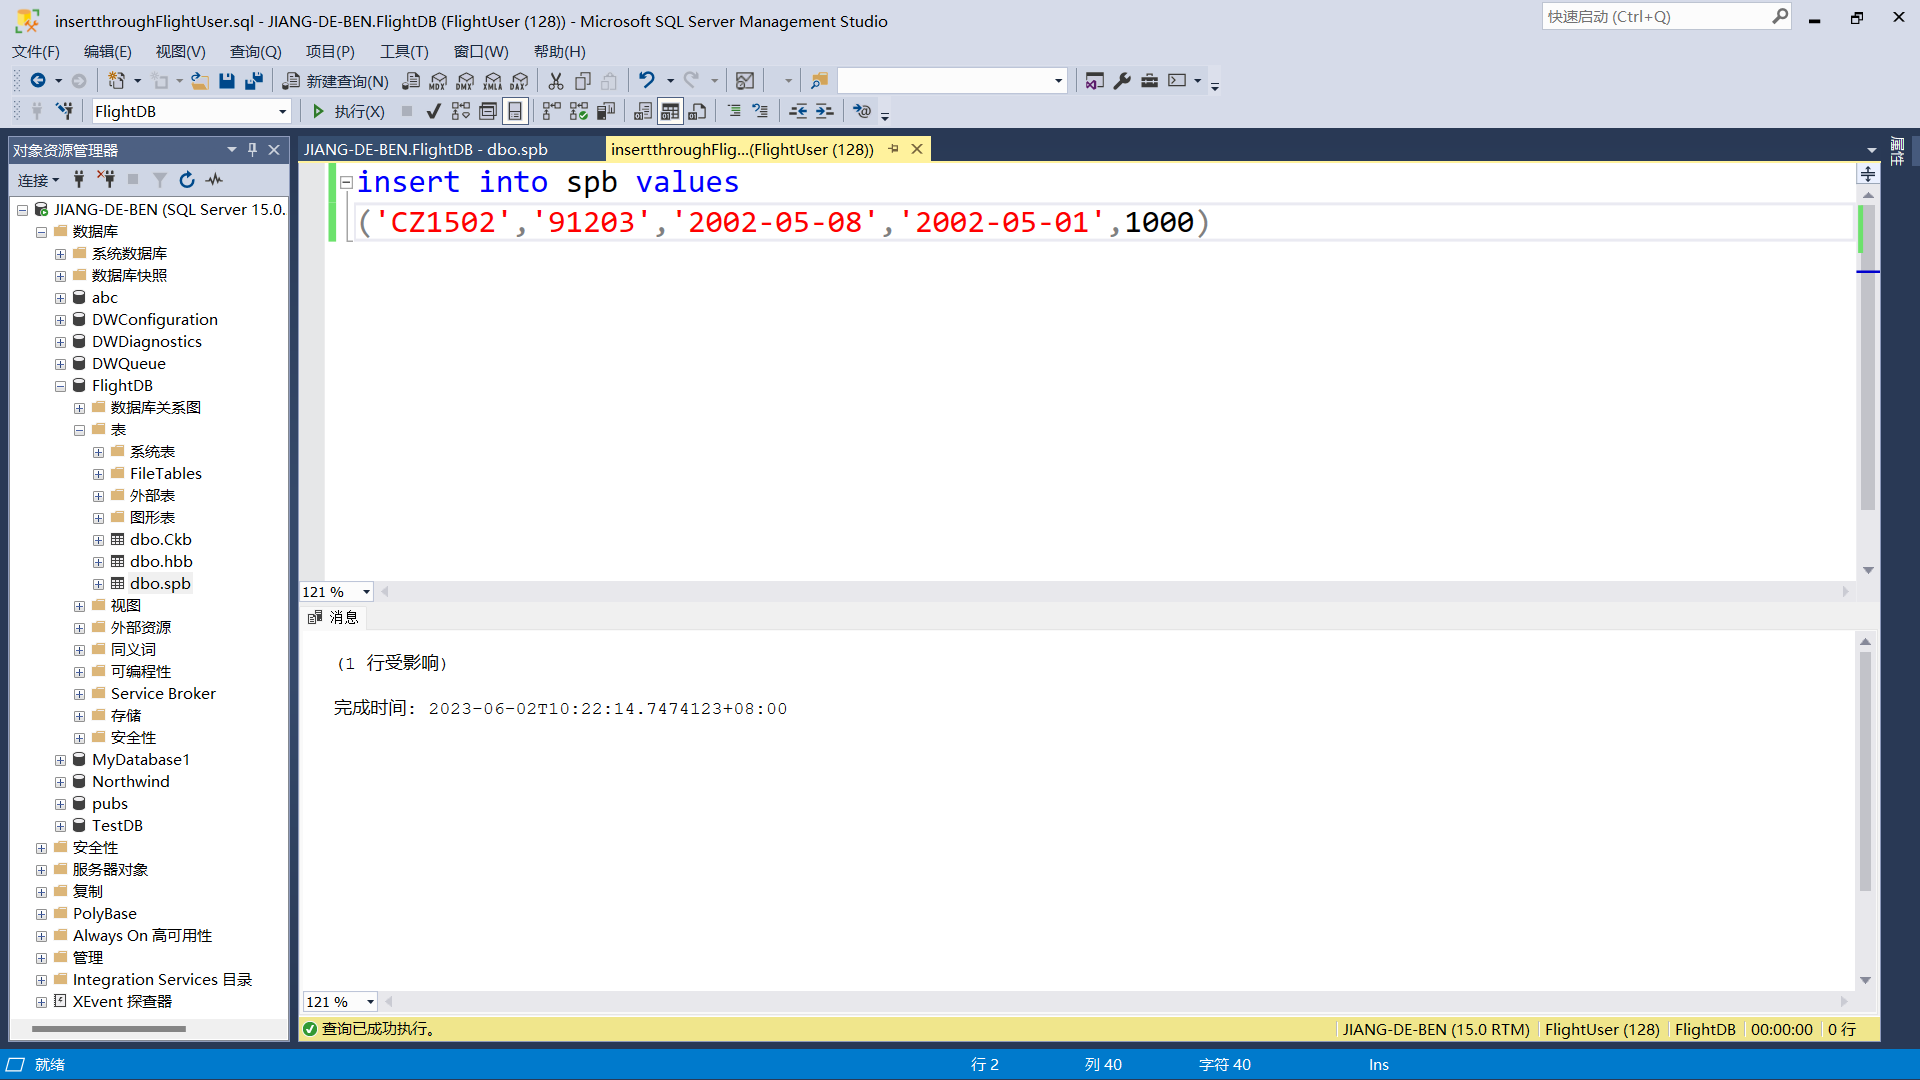
\includegraphics[width=0.9\linewidth]{img/16.png}
    \end{minipage}
    \caption{FlightUser权限验证}
\end{figure}

\section{实验总结}
本次实验主要是对SQL Server的使用,通过对SQL Server的DDL、DML、备份、还原、权限分配等功能的使用,对SQL Server有了更深入的了解,同时也对数据库的基本操作有了更深入的认识。

在实验的过程中,我发现SQL Server的GUI界面操作非常方便,可以直观的看到操作的结果,同时也可以直接生成对应的SQL语句,方便了SQL语句的编写,提高了效率。

但是,使用代码实现的方式更加灵活,可以实现更多的功能,同时也可以更好的理解SQL语句的执行过程,所以在实际的使用中,我会更多的使用代码实现的方式。
















    


\end{document}